\documentclass[a4paper, 11pt]{article}

\usepackage[english]{babel}
\usepackage[utf8]{inputenc}
\usepackage[T1]{fontenc}
\usepackage{placeins}
\usepackage{qtree}
\usepackage{csquotes}
\usepackage{hyperref}
\usepackage{amsmath}
\usepackage{tikz}
\usepackage{tikz-uml}
\usepackage{multicol}
\usetikzlibrary{automata,arrows,positioning,shapes}
\usepackage{graphicx}
\usepackage{amsmath}
\usepackage[left=2cm,right=2cm,top=2cm,bottom=2cm]{geometry}

\graphicspath{{img/}}

\author{Florian Thuin (SINF21MS/G) 06561100 \and Nicolas Houtain (SINF22MS/G) 69801100}
\date{\today}
\title{Software engineering: Development methods --- Assignment 2}

\begin{document}

    \maketitle
    \tableofcontents
    \clearpage{}

    \section{Architectural design}
    \subsection{Decomposition hierarchical view}

    \noindent
    \begin{tikzpicture}
        \begin{umlpackage}{Client}
            \umlclass{Gas pump interface}{}{}
            \umlclass[y=-3]{Credit card reader}{}{}
        \end{umlpackage}
        \begin{umlpackage}[x=6]{System}
            \begin{umlpackage}{GUI}
                \umlclass{Cashier's interface}{}{}
            \end{umlpackage}
            \begin{umlpackage}[y=-3]{Controller}
                \umlclass{Gas pump controller}{}{}
                \umlclass[y=-2]{Credit card controller}{}{}
                \umlclass[y=-4]{Purchase controller}{}{}
            \end{umlpackage}
            \begin{umlpackage}[x=6]{Logger}
                \umlclass{Accounting inventory}{}{}
                \umlclass[y=-2]{Fuel stock inventory}{}{}
            \end{umlpackage}
        \end{umlpackage}
    \end{tikzpicture}

    \noindent
    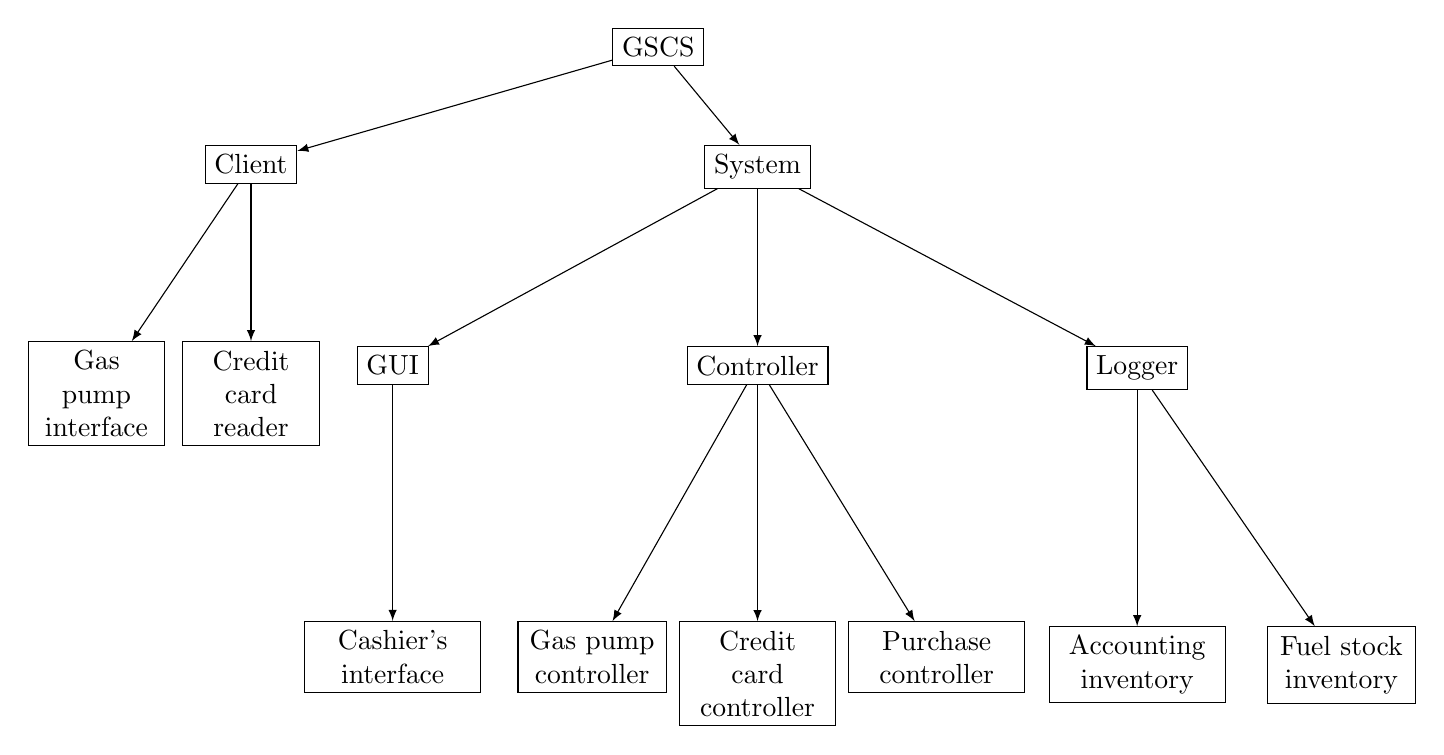
\begin{tikzpicture}
        \node[draw] (GSCS) {GSCS};
        \node[draw, below left = 1cm and 4cm of GSCS] (Client) {Client};
        \node[draw, below left = 2cm and 0.5cm of Client, text width=1.5cm, align=center] (GPI) {Gas pump interface};
        \node[draw, below = 2cm of Client, text width=1.5cm, align=center] (CCR) {Credit card reader};
        \node[draw, below right = 1cm and 0cm of GSCS] (System) {System};
        \node[draw, below left = 2cm and 3.5cm of System] (GUI) {GUI};
        \node[draw, below = 3cm of GUI, text width=2cm, align=center] (CI) {Cashier's interface};
        \node[draw, below = 2cm of System] (Controller) {Controller};
        \node[draw, below left = 3cm and 0.25cm of Controller, text width=1.65cm, align=center] (GPC) {Gas pump controller};
        \node[draw, below = 3cm of Controller, text width=1.75cm, align=center] (CCC) {Credit card controller};
        \node[draw, below right = 3cm and 0.25cm of Controller, text width=2cm, align=center] (PC) {Purchase controller};
        \node[draw, below right = 2cm and 3.5cm of System] (Logger) {Logger};
        \node[draw, below = 3cm of Logger, text width=2cm, align=center] (AI) {Accounting inventory};
        \node[draw, below right = 3cm and 1cm of Logger, text width=1.65cm, align=center] (FSI) {Fuel stock inventory};

        \path[-latex] (GSCS) edge node {} (Client);
        \path[-latex] (GSCS) edge node {} (System);
        \path[-latex] (Client) edge node {} (GPI);
        \path[-latex] (Client) edge node {} (CCR);
        \path[-latex] (System) edge node {} (GUI);
        \path[-latex] (System) edge node {} (Controller);
        \path[-latex] (System) edge node {} (Logger);
        \path[-latex] (GUI) edge node {} (CI);
        \path[-latex] (Controller) edge node {} (GPC);
        \path[-latex] (Controller) edge node {} (CCC);
        \path[-latex] (Controller) edge node {} (PC);
        \path[-latex] (Logger) edge node {} (AI);
        \path[-latex] (Logger) edge node {} (FSI);
    \end{tikzpicture}

    \subsection{Roles and interactions}

    The components are separated in two main parts: the client and the system.

    \subsubsection{Client}

    The client contains the modules directly related to the
    customer that contains:

    \begin{description}
        \item[Gas pump interface:] This graphical user interface is in charge of
        displaying information sent by the system and sending back input from
        the customer. As it is said in the assignment, the communication is
        handled by external libraries.
        \item[Credit card reader:] This module is in charge of retrieving and
        sending the credit card number or an error to the system. The
        communication is handled by external libraries.
    \end{description}

    \subsubsection{System}

    The system contains the modules directly related to the management of the
    data of the parts of the GSCS or from the cashier. There are three main
    sub-modules that have components:

    \begin{description}
        \item[GUI:] The graphical user interface inside the system
            \subitem\textbf{Cashier's interface} The cashier's interface is a
            GUI that displays information from the purchase controller to the
            cashier.
        \item[Controller:] Input and commands handler
            \subitem\textbf{Gas pump controller} handles the data from the gas
            pump and the gas pump interface, sends messages to the gas pump
            interface and sends information to the purchase controller.
            \subitem\textbf{Credit card controller} handles the data from the
            credit card reader, sends error to the gas pump controller if any
            or sends confirmation/error to the purchase controller.
            \subitem\textbf{Purchase controller} handles the data from the gas
            pump controller, sends information to the credit card controller
            and the cashier's interface and queries the logger's modules when
            the current purchase is done.
        \item[Logger:] DBMS to retrieve or modify stored data
            \subitem\textbf{Accounting inventory} stores and retrieves data
            related to customer billing account.
            \subitem\textbf{Fuel stock inventory} stores and retrieves data
            related to the amount purchased at each gas pump.
    \end{description}

    \section{Detailed design}
    \subsection{Class diagram}

    \newgeometry{left=0.5cm, bottom=0.5cm}
    \tikzumlset{font=\scriptsize}
    \begin{tikzpicture}[on grid, auto]
        \umlclass[x=1]{Purchase}{+amount: float \\ +price: float}{+isFinished(): boolean}
        \umlsimpleclass[x=10]{Fuel}
        \umlclass[x=14]{Fuel stock}{+amount: float \\ +capacity: float}{}
        \umlsimpleclass[x=-1,y=-3]{Cash purchase}
        \umlsimpleclass[x=1,y=-4]{Account purchase}
        \umlsimpleclass[x=3,y=-3]{Credit purchase}
        \umlclass[x=8.5, y=-2]{Gas pump}{+id: int}{+reportPurchase(): Purchase}
        \umlclass[x=10, y=-8]{Gas pump controller}{}{+sendMessage(message:String): void\\ +handlePaymentOption(): void}
        \umlclass[x=14,y=-3]{Gas pump interface}{+pumpNumber: int}{+displayText(message:String):void\\ +reset(): void\\ +transmitOption():int}
        \umlclass[x=15,y=-5.5]{Credit card reader}{+pumpNumber: int}{+getCardNumber(): String}
        \umlclass[x=7,y=-5]{Credit transaction}{+cardNumber: String\\ +price: float}{}
        \umlclass[x=10,y=-13]{Controller}{}{+handlePayment(payment:Payment): void\\ +handlePurchase(purchase: Purchase): void\\ +isCustomerRegistered(): boolean}
        \umlclass[y=-7]{Account}{+number: String\\ +balance:float}{}
        \umlclass[x=10,y=-17]{Cashier's interface}{}{+backToPreviousScreen(): View\\ +displayText(message:String)\\ +transmitOption(): int\\ +transmitInput(): String}
        \umlclass[x=10,y=-21]{Cashier}{+cash: float}{+performMaintenance(): void\\ +registerCustomer(name:String,address:String,phoneNumber:String): void\\ +chooseOption(): void\\ +monthlyBillPayment(billingAccountNumber:String,dollarsAmount:float): void\\ +handleCashPayment(dollarsAmount:float): void\\ +input(): text}
        \umlclass[y=-14]{Customer}{+name: String\\ +address: String\\ +phoneNumber: String\\ +accountNumber: String}{+choosePaymentOption(): void\\ +swipeCard(): void\\ +payCash(): void}
        \umlclass[x=3,y=-7]{Payment}{+price: float\\ +date: Date}{}
        \umlsimpleclass[x=1,y=-10]{Check payment}
        \umlsimpleclass[x=4.5,y=-10]{Credit payment}
        \umlclass[x=14,y=-10]{Credit card system}{}{+reimburse(payment:Payment):boolean}

        \umlinherit[geometry=|-|, anchor1=90, anchor2=230]{Cash purchase}{Purchase}
        \umlinherit{Account purchase}{Purchase}
        \umlinherit[geometry=|-|, anchor1=90, anchor2=310]{Credit purchase}{Purchase}
        \umlassoc[mult1=0..*,mult2=1,align1=left, align2=left]{Purchase}{Fuel}
        \umlassoc[mult1=1,mult2=1]{Fuel}{Fuel stock}
        \umlinherit[geometry=|-|, anchors=60 and -135]{Check payment}{Payment}
        \umlinherit[geometry=|-|, anchors=60 and -45]{Credit payment}{Payment}
        \umlassoc{Payment}{Account}
        \umlassoc[geometry=|-|, anchor1=220, anchor2=-135,mult1=0..1,mult2=1,pos2=2.2]{Account}{Customer}
        \umlassoc[geometry=|-|,mult1=1,mult2=0..*,pos2=2.7]{Account}{Account purchase}
        \umlassoc[anchor2=30,mult1=1,mult2=0..1]{Credit transaction}{Credit payment}
        \umlassoc[mult1=1,mult2=1]{Cashier}{Cashier's interface}
        \umlassoc[mult1=1,mult2=1]{Controller}{Cashier's interface}
        \umlassoc[mult1=1,mult2=1..*,pos1=0.4]{Controller}{Credit card system}
        \umlassoc[mult1=1,mult2=1..*]{Controller}{Gas pump controller}
        \umlassoc[mult1=1,mult2=1,pos1=0.6]{Gas pump controller}{Credit card reader}
        \umlassoc[mult1=1,mult2=1]{Gas pump controller}{Gas pump interface}
        \umlassoc[mult1=1,mult2=1]{Gas pump controller}{Gas pump}
        \umlassoc[mult1=1,mult2=0..*]{Gas pump}{Purchase}
        \umlassoc[mult1=1,mult2=0..1,pos1=0,pos2=0.5]{Credit transaction}{Credit purchase}
    \end{tikzpicture}
    \restoregeometry

    \subsubsection{Short description of the roles of the class}

    \begin{description}
        \item[Fuel stock] reifies the inventory, it is the object that models
        the database.
        \item[Fuel] is a companion object that makes the link between a purchase
        and the database.
        \item[Purchase] reifies a purchase and is a superclass for every kind of
        purchase.
        \item[Cash purchase] reifies a purchase paid by cash.
        \item[Credit purchase] reifies a purchase paid by credit card.
        \item[Account purchase] reifies a purchase paid with monthly billing.
        \item[Gas pump] reifies a single gas pump.
        \item[Gas pump interface] reifies a single gas pump interface.
        \item[Credit card reader] reifies a single credit card reader.
        \item[Credit transaction] reifies a single credit transaction.
        \item[Gas pump controller] is an helper that manages in one place every
        part of the pump (the pump, the interface, the card reader) for sending
        data to/receiving data from the system.
        \item[Account] contains data following the requirements.
        \item[Payment] reifies a monthly bill payment.
        \item[Check payment] reifies a payment for a monthly bill made by check.
        \item[Credit payment] reifies a payment for a monthly bill made by credit card.
        \item[Customer] reifies a customer following the given requirements.
        \item[Credit card system] reifies the credit card system following the given
        requirements.
        \item[Controller] is an helper that manages in one place all the gas pump controllers,
        the single cashier interface and the credit card system to easily transmit
        data between those parts of the system.
        \item[Cashier's interface] reifies the cashier's interface following the given
        requirements.
        \item[Cashier] reifies a cashier following the given requirements.
    \end{description}

    \subsection{Uses diagram}

    \newgeometry{left=0.5cm, bottom=0.5cm}
    \tikzumlset{font=\scriptsize}
    \begin{tikzpicture}[on grid, auto]
        \umlclass[x=1]{Purchase}{+amount: float \\ +price: float}{+isFinished(): boolean}
        \umlsimpleclass[x=10]{Fuel}
        \umlclass[x=14]{Fuel stock}{+amount: float \\ +capacity: float}{}
        \umlsimpleclass[x=-1,y=-3]{Cash purchase}
        \umlsimpleclass[x=1,y=-4]{Account purchase}
        \umlsimpleclass[x=3,y=-3]{Credit purchase}
        \umlclass[x=8.5, y=-2]{Gas pump}{+id: int}{+reportPurchase(): Purchase}
        \umlclass[x=10, y=-8]{Gas pump controller}{}{+sendMessage(message:String): void\\ +handlePaymentOption(): void}
        \umlclass[x=14,y=-3]{Gas pump interface}{+pumpNumber: int}{+displayText(message:String):void\\ +reset(): void\\ +transmitOption():int}
        \umlclass[x=15,y=-5.5]{Credit card reader}{+pumpNumber: int}{+getCardNumber(): String}
        \umlclass[x=7,y=-5]{Credit transaction}{+cardNumber: String\\ +price: float}{}
        \umlclass[x=10,y=-13]{Controller}{}{+handlePayment(payment:Payment): void\\ +handlePurchase(purchase: Purchase): void\\ +isCustomerRegistered(): boolean}
        \umlclass[y=-7]{Account}{+number: String\\ +balance:float}{}
        \umlclass[x=10,y=-17]{Cashier's interface}{}{+backToPreviousScreen(): View\\ +displayText(message:String)\\ +transmitOption(): int\\ +transmitInput(): String}
        \umlclass[x=10,y=-21]{Cashier}{+cash: float}{+performMaintenance(): void\\ +registerCustomer(name:String,address:String,phoneNumber:String): void\\ +chooseOption(): void\\ +monthlyBillPayment(billingAccountNumber:String,dollarsAmount:float): void\\ +handleCashPayment(dollarsAmount:float): void\\ +input(): text}
        \umlclass[y=-14]{Customer}{+name: String\\ +address: String\\ +phoneNumber: String\\ +accountNumber: String}{+choosePaymentOption(): void\\ +swipeCard(): void\\ +payCash(): void}
        \umlclass[x=3,y=-7]{Payment}{+price: float\\ +date: Date}{}
        \umlsimpleclass[x=1,y=-10]{Check payment}
        \umlsimpleclass[x=4.5,y=-10]{Credit payment}
        \umlclass[x=14,y=-10]{Credit card system}{}{+reimburse(payment:Payment):boolean}

        \umlimport{Cash purchase}{Purchase}
        \umlimport{Account purchase}{Purchase}
        \umlimport{Credit purchase}{Purchase}
        \umlimport{Account}{Payment}
        \umlimport{Check payment}{Payment}
        \umlimport{Credit payment}{Payment}
        \umlimport[anchor1=120, anchor2=-135]{Customer}{Account}
        \umlimport{Credit transaction}{Credit purchase}
        \umlimport{Gas pump controller}{Gas pump interface}
        \umlimport{Gas pump controller}{Credit card reader}
        \umlimport{Gas pump controller}{Gas pump}
        \umlimport{Gas pump}{Purchase}
        \umlimport{Purchase}{Fuel}
        \umlimport{Fuel}{Fuel stock}
        \umlimport{Controller}{Cashier's interface}
        \umlimport{Controller}{Credit card system}
        \umlimport{Controller}{Gas pump controller}
        \umlimport[anchor1=155, anchor2=-120]{Controller}{Credit transaction}
        \umlimport{Controller}{Customer}
        \umlimport{Cashier's interface}{Cashier}
    \end{tikzpicture}
    \restoregeometry

    \subsubsection{Incremental development}

    \begin{enumerate}
        \item Design and create the databases
        \item Develop the user's interfaces
        \item Develop the utilities (account, customer, payment, cashier,\ldots)
        \item Develop the controllers
    \end{enumerate}

    \section{Design patterns}
    \subsection{Template pattern}

    \begin{tikzpicture}
        \umlclass[type=abstract,x=1]{Payment}{+price: float\\ +date: Date}{+getReceipt(): void\\ \textit{-getPaymentMethodName(): String}}
        \umlclass[y=-4]{Check payment}{}{-getPaymentMethodName(): String}
        \umlclass[x=6,y=-4]{Credit payment}{}{-getPaymentMethodName(): String}

        \umlnote[x=10,width=9cm]{Payment}{abstract class Payment \{ \\
                                          \ \ \ \ float price; \\
                                          \ \ \ \ Date date; \\

                                          \ \ \ \ public String getReceipt() \{ \\
                                          \ \ \ \ \ \ \ \ String result = "DINOCO " + date.toString() + "\textbackslash{}n"; \\
                                          \ \ \ \ \ \ \ \ result += "Price: " + price; \\
                                          \ \ \ \ \ \ \ \ result += "paid with " + getPaymentMethodName(); \\
                                          \ \ \ \ \ \ \ \ return result; \\
                                          \ \ \ \ \} \\
                                          \ \ \ \ private abstract String getPaymentMethodName(); \\
                                \}}
        \umlnote[x=12,y=-4, width=5.5cm]{Credit payment}{private String getPaymentMethodName \{ \\
                                                       \ \ \ \ return "credit card"; \\
                                                       \}}
        \umlnote[y=-6, width=5.5cm]{Check payment}{private String getPaymentMethodName \{ \\
                                                       \ \ \ \ return "check"; \\
                                      \}}

        \umlinherit{Check payment}{Payment}
        \umlinherit{Credit payment}{Payment}
    \end{tikzpicture}
    \subsection{Strategy pattern}

    \begin{tikzpicture}
        \umlclass{PrintOut}{reporting:Reporting}{print(): void}
        \umlclass[type=interface,x=7]{Reporting}{}{\textit{+print(): void}}
        \umlclass[x=4,y=-3]{Payment}{+price: float\\ +date: Date}{+print(): void}
        \umlclass[x=10,y=-3]{Account}{+number: String\\ +balance: float}{+print(): void}
        \umlsimpleclass[x=2,y=-5.5]{Check payment}
        \umlsimpleclass[x=6,y=-5.5]{Credit payment}

        \umlimpl[geometry=|-|, anchor2=-110]{Payment}{Reporting}
        \umlimpl[geometry=|-|, anchor2=-70]{Account}{Reporting}
        \umlinherit[geometry=|-, anchor2=-150]{Check payment}{Payment}
        \umlinherit[geometry=|-, anchor2=-30]{Credit payment}{Payment}
        \umlassoc{Payment}{Account}
        \umlcompo{PrintOut}{Reporting}

        \umlnote[x=12]{Reporting}{public void print();}
        \umlnote[x=12,y=-9, width=8cm]{Account}{public class Account implements Reporting \{ \\
                                     \ \ \ \ public String number = ""; \\
                                     \ \ \ \ public float balance = 0.0; \\
                                     \ \ \ \ ... \\
                                     \ \ \ \ public void print() \{ \\
                                     \ \ \ \ \ \ \ \ ... \\
                                     \ \ \ \ \ \ \ \ System.out.println("Account number: " + number); \\
                                     \ \ \ \ \ \ \ \ ... \\
                                     \ \ \ \ \ \ \ \ System.out.println("Account balance: " + balance); \\
                                     \ \ \ \ \ \ \ \ ... \\
                                     \ \ \ \ \} \\
                                     \ \ \ \ ... \\
                                     \}}
        \umlnote[x=3.5,y=-9, width=8cm]{Payment}{public class Payment implements Reporting \{ \\
                                                \ \ \ \ public float price = 0.0; \\
                                                \ \ \ \ public Date date = new Date(); \\
                                                \ \ \ \ ... \\
                                                \ \ \ \ public void print() \{ \\
                                                \ \ \ \ \ \ \ \ ... \\
                                                \ \ \ \ \ \ \ \ System.out.println("Date: " + date.toString()); \\
                                                \ \ \ \ \ \ \ \ ... \\
                                                \ \ \ \ \ \ \ \ System.out.println("Price: " + price); \\
                                                \ \ \ \ \ \ \ \ ... \\
                                                \ \ \ \ \} \\
                                                \ \ \ \ ... \\
                                                \}}
        \umlnote[y=-2.5, width=4cm]{PrintOut}{public void print() \{ \\
                           \ \ \ \ return reporting.print(); \\
                          \}}
    \end{tikzpicture}

    \subsection{Decorator pattern}

    \begin{tikzpicture}
        \umlclass[type=interface]{Purchase}{+amount: float\\ +price:float}{\textit{+isFinished(): boolean}\\ \textit{getPrice(): float}}
        \umlclass[x=6, y=-2]{PurchaseDecorator}{+amount: float\\ +price: float\\ +purchase: Purchase}{+isFinished(): boolean\\ +getPrice(): float}
        \umlclass[x=8, y=-6]{Credit purchase}{+fee: float}{-processFee(): float\\ +getPrice(): float}
        \umlclass[y=-6]{Cash purchase}{}{+isFinished(): boolean\\ +getPrice(): float}
        \umlclass[x=4, y=-6]{Account purchase}{}{+isFinished(): boolean\\ +getPrice(): float}

        \umlcompo[geometry=|-]{PurchaseDecorator}{Purchase}
        \umlimpl{PurchaseDecorator}{Purchase}
        \umlimpl{Cash purchase}{Purchase}
        \umlimpl{Account purchase}{Purchase}
        \umlinherit{Credit purchase}{PurchaseDecorator}

        \umlnote[x=11,y=-2, width=4cm]{PurchaseDecorator}{public float getPrice() \{ \\
                                    \ \ \ \ return purchase.getPrice(); \\
                                   \}}
        \umlnote[x=12.5, y=-6, width=4.5cm]{Credit purchase}{public float getPrice() \{ \\
                                              \ \ \ \ return processFee() + price; \\
                                             \}}
    \end{tikzpicture}

    \subsection{Observer pattern}

    \begin{tikzpicture}
        \umlclass[type=abstract]{Observable}{-listOfObservers: List<Observer>}{+register(observer:Observer): void\\ +unregister(observer:Observer): void\\ +notifyAll(): void}
        \umlclass[y=-3]{Gas pump}{+id: int}{+reportPurchase(): Purchase}
        \umlclass[y=-6]{Purchase}{+amount: float\\ +price: float}{+isFinished(): boolean}
        \umlclass[type=interface,x=6,y=-3]{Observer}{}{+notify(purchase:Purchase):void}
        \umlclass[x=6,y=-6]{Controller}{}{+handlePayment(payment:Payment): void\\ +handlePurchase(purchase:Purchase): void\\ +isCustomerRegistered(): boolean\\ +notify(purchase:Purchase): void}
        \umlclass[x=12,y=-3]{Fuel stock}{+amount: float\\ +capacity: float}{+notify(purchase:Purchase): void}

        \umlimpl{Fuel stock}{Observer}
        \umlimpl{Controller}{Observer}
        \umlassoc{Purchase}{Gas pump}
        \umlaggreg{Gas pump}{Observer}
        \umlinherit{Gas pump}{Observable}

        \umlnote[x=7, width=5.5cm]{Observable}{public void notifyAll() \{ \\
                                 \ \ \ \ for (Observer o : listOfObservers) \{ \\
                                 \ \ \ \ \ \ \ \ o.notify(purchase); \\
                                 \ \ \ \ \} \\
                                 \}}
        \umlnote[x=4,y=-9, width=5.5cm]{Controller}{public void notify(Purchase purchase) \{ \\
                                  \ \ \ \ handlePurchase(purchase); \\
                                  \}}
        \umlnote[x=11,y=-9, width=5.5cm]{Fuel stock}{public void notify(Purchase purchase) \{ \\
                                                  \ \ \ \ this.amout -= purchase.amount; \\
                                                 \}}
    \end{tikzpicture}

    \subsection{Composite pattern}

    \begin{tikzpicture}
        \umlclass[type=interface,x=4]{Account}{}{+getBalance(): float}
        \umlclass[y=-3]{SingleAccount}{+number: String\\ +balance: float}{+getBalance(): float}
        \umlclass[y=-7]{Customer}{+name: String\\ +address: String\\ +phoneNumber: String\\ +accountNumber: String}{+choosePaymentOption(): void\\ +swipeCard():void\\ +payCash(): void}
        \umlclass[x=8,y=-3]{CompanyAccount}{+accounts: List<Account>}{+add(account:Account): void\\ +remove(account:Account): void\\ +getBalance(): float)}

        \umlimpl{SingleAccount}{Account}
        \umlimpl{CompanyAccount}{Account}
        \umlassoc[mult1=1, mult2=0..1]{Customer}{SingleAccount}
        \umlaggreg[geometry=|-]{CompanyAccount}{Account}

        \umlnote[width=4cm]{SingleAccount}{public float getBalance() \{ \\
                                \ \ \ \ return balance; \\
                               \}}
        \umlnote[width=5cm,x=8, y=-7]{CompanyAccount}{public float getBalance() \{ \\
                                                \ \ \ \ float res = 0.0; \\
                                                \ \ \ \ for (Account a : accounts) \{ \\
                                                \ \ \ \ \ \ \ \ res += a.getBalance(); \\
                                                \ \ \ \ \} \\
                                                \ \ \ \ return res; \\
                                                \}}
    \end{tikzpicture}
\end{document}
